\chapter{实例抽取与关系挖掘}
\section{目标}
对于一项活动,除了抽象的活动概念以外,还应有相应的属性,如情感状态、时间、地点。为此,我们定义了活动实例(定义\ref{def:instance}。本章的目标在于,输入一条特定微博$m$, 从中抽取活动相关属性,构建活动的实例$a$;并基于实例抽取的结果,进一步构建活动之间的关系。

\section{活动类别抽取}

在第\ref{chp:concept}中,我们已经抽取出一系列抽象的活动概念。在构建活动实例时,我们首先要获取微博$m$对应的活动概念,即活动类别抽取。

类似于第\ref{chp:concept}章的方法,本文首先使用了规则匹配,首先抽取微博中所有的动词短语,并判断是不是对应一个活动概念,这一步只需判断它是否在抽取出的活动概念集合即可。如果不存在,则认为这条微博包含一个活动。这样做的结果精度为74\%,但召回率仅为56\%。对结果的分析发现,大约有11\%的缺失是由于语法结构的复杂性。用户在表述一项活动时,动作和目标有时并不构成一个简单的动宾短语,例如以下情况
\begin{itemize}
\item 宾语可以前置,如``找本书读了一下午'',
\item 加入复杂的修饰成分,如``陪父母看了一场周星驰拍的很有意思的电影''
\item 以主谓、定中等形式出现。如``练了一天的琴''。
\end{itemize}
这些较复杂的情况,通过简单的词法分析和规则匹配是难以处理的。为解决这个问题,本文对句子进行句法分析,将线性文本处理为依存树。句法分析在当前已有许多成熟的分析器,如Stanford Parse\footnote{http://nlp.stanford.edu/software/lex-parser.shtml}和HIT-LTP\footnote{http://www.ltp-cloud.com/}。

Stanford Parser是斯坦福大学自然语言处理组开发的句法分析工具。它主要面向英语语言,也提供中文、德语、阿拉伯语等其他语种的解析,但它的处理结果并不非常直观。最终本文选择哈尔滨工业大学开源的语言技术平台(Language Technology Platform, LTP)\cite{che2010ltp}作为句法分析工具。LTP提供分词、词性标注、命名实体识别、依存句法分析、语义角色标注等功能,提供自然语言处理的集成解决方案。LTP接收原始文本作为输入,结果以XML的形式给出,对每个词,给出其依赖词和依赖关系,依赖关系包括主谓(SBV),动宾(VOB), 定中(ATT),并列(COO)等。图\ref{fig:ltp_demo}是LTP进行句法分析的结果,它正确分析出``看''和``电影''的动宾关系。

\begin{figure}[!h]
\centering
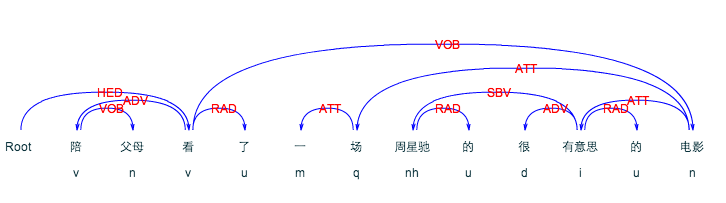
\includegraphics[width=0.9\textwidth]{ltpdemo1.png}
\caption{LTP句法分析示例}
\label{fig:ltp_demo}
\end{figure}

通过LTP进行句法分析,得到词语之间的依赖关系,进一步抽出动词短语,判断是否是一个活动概念,结果如表\ref{table:cat_extraction}。

\begin{table}
\centering
\begin{tabular}{|c|c|c|c|}
\hline
& Precision & Recall & F1 score \\
\hline
Result & 73.2\% & 68.4 \% & 0.707 \\ 
\hline
\end{tabular}
\caption{活动类别抽取实验结果}
\label{table:cat_extraction}
\end{table}

除精度、召回率以外,处理速度也是一个关键的问题。将整条微博作为LTP的输入,处理速度非常慢,分析工作的复杂度随文本长度指数增长。为提高速度,首先将文本分割为多个短句,再进行分析,就可以达到较快的速度。由于不同微博的分析工作是独立的,为了进一步提高处理能力,可以使用多线程、多机进行并发。图\ref{fig:parse_speed}中比较了不同处理策略,分析1000条微博的速度。

\begin{figure}[!h]
\centering
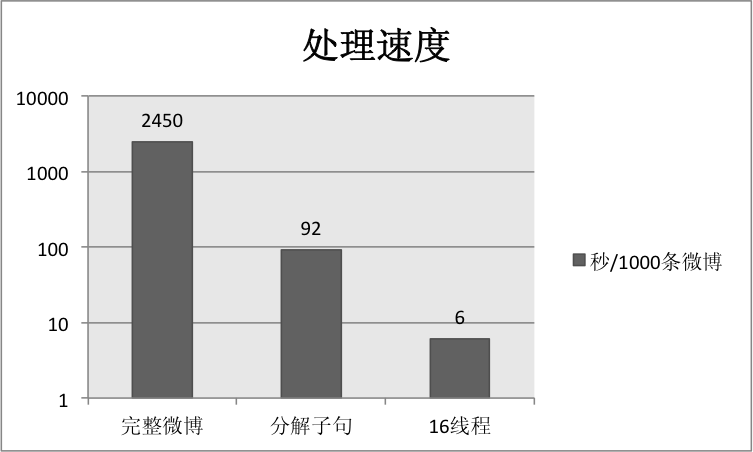
\includegraphics[width=0.7\textwidth]{speed.png}
\caption{分析速度}
\label{fig:parse_speed}
\end{figure}

本文方法的不足在于,没有考虑特定命名实体与活动类别的关系。如,``下午去看了阿凡达''这类微博。``阿凡达''是一部电影的名称,因此这条微博应对应``看电影''这个活动类别,但本文的方法无法正确抽取这类活动。类似的情况如餐馆、电视剧、特定的地名等等。在下一步工作中,可以引入外部的知识库,以建立命名实体与活动的联系。

\section{情感极性分析}
在活动抽取中,如果微博中包含用户参与的一项活动,我们希望了解用户参与这项活动时的心情状态如何,帮助我们发现活动本身是正面还是负面,这样帮助推荐系统进行选择。因此,需要获取微博的情感极性。

\subsection{方法概述}
本文的工作中,对微博进行三分类,正面(positive),中性(neutral)和负面(negative)。

我们对非监督和监督学习均进行了尝试。在非监督的方法中,我们从知网(Hownet)等途径获取了中文的情感词典,共有4986个积极词汇和4818个消极词汇,包含动词、形容词和名词。对每一条微博,我们首先计算计算其中积极、消极词汇的数量$n_{pos}$和$n_{neg}$,若其差值$|n_{pos}-n_{neg}|<\theta$,则认为微博是中性的,否则判别为词数多的类别。但这样简单的非监督方法只能达到55\%的正确率(注意到这是三分类问题,这个结果还是比随机分类(33\%)和全部判为最多的类别(45\%)要好)。为此,我们使用监督学习的方法,使用以下特征训练分类器

\begin{enumerate}
\item Bigrams和Unigrams的频度。使用bigram的原因是,情感词之前常常会带有修饰性的前缀,如``不'',``非常'',有时会加强或者逆转情感词的极性。因此对于较频繁出现的模式,是哟高bigram作为特征。
\item 正面词、负面词出现的频度。这可以根据情感词典得到。
\item 表情符号。用户在发布微博时,常常会加入一些表情,如``高兴'',``愤怒'',有时用户选择表情并不关心这个表情具体的含义是什么,但是也可以体现出用户当时的心理状态。
\end{enumerate}
同时,为了加快训练速度和减少噪声,我们将过于稀疏,即出现次数少于一个下界的特征滤除。

\subsection{实验结果与分析}
我们标注了20829条包含活动信息的微博,根据其情感极性标注为5级,-2为很负面,-1为一般负面,0为中性,1为一般积极,2为很积极,其中分级-2、-1为负面,+1,+2为中性,0为中性。为了避免不同人倾向性的不同,每条微博会有至少两个人标注,如果出现分歧,由实验者最终决定类别。在数据中,共有9462条为中性,6566条为正面,4787条为负面。在此数据上进行交叉验证。

我们首先检验不同特征的选取对分类精度的影响,如图\ref{fig:sentiment_feature}。可以看到,我们选取的特征,对于分类结果都有明显的提升,其中情感词词典的作用最为明显。
\begin{figure}[!h]
\centering
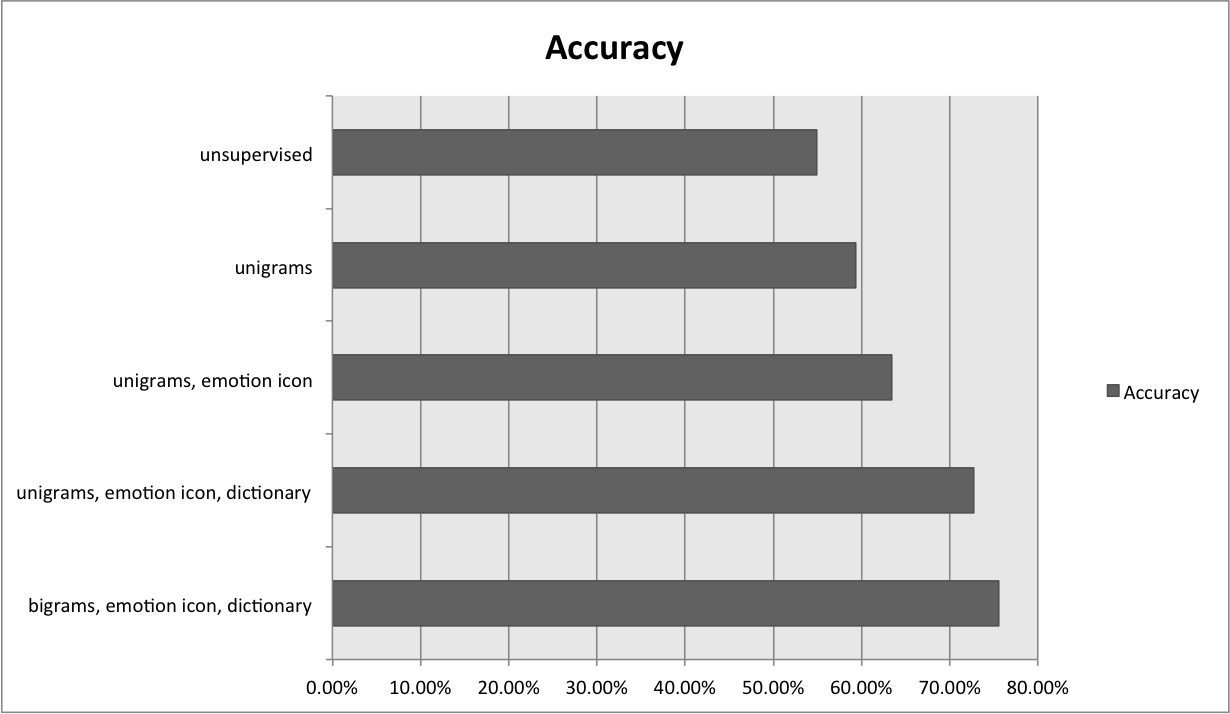
\includegraphics[width=0.9\textwidth]{sentiment_feature.png}
\caption{特征选择}
\label{fig:sentiment_feature}
\end{figure}

本文继续尝试了不同的分类模型,包括
\begin{itemize}
\item 朴素贝叶斯
\item 以决策树为基础的AdaBoost
\item 随机森林
\item 线性核SVM
\end{itemize}
测试结果如图\ref{fig:sentiment_model}。线性核SVM表现最好,但朴素贝叶斯也有比较好的性能,与\cite{pang2002thumbs}中的结果一致。

\begin{figure}[!h]
\centering
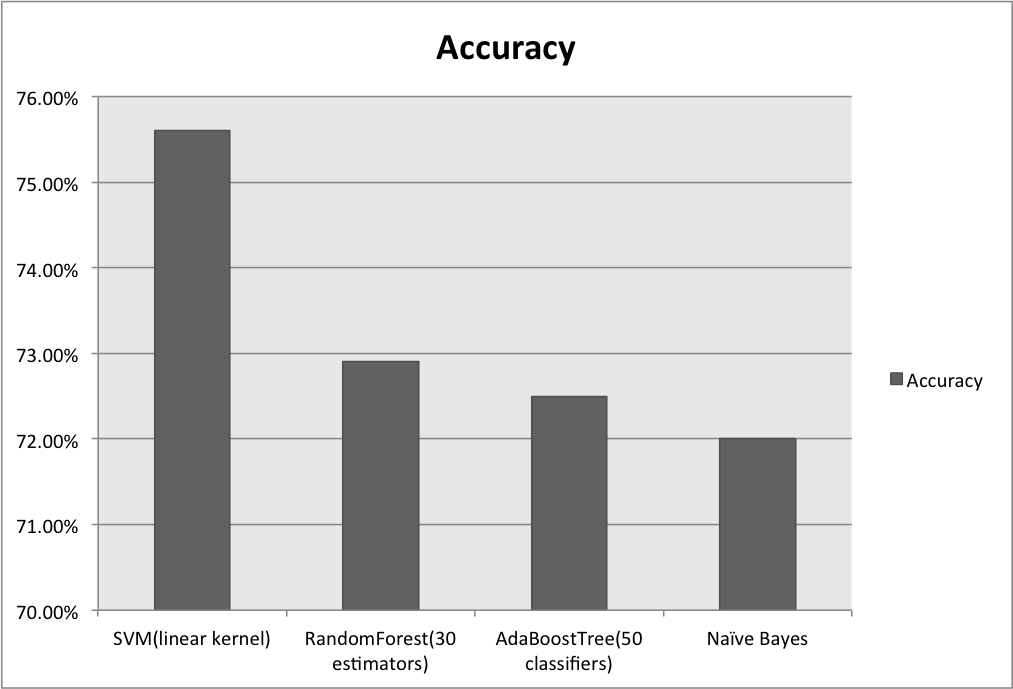
\includegraphics[width=0.8\textwidth]{sentiment_model.png}
\caption{模型选择}
\label{fig:sentiment_model}
\end{figure}

最终达到的75\%的分类精度从数值上看并不是很高,但情感极性的判断有很强的主观性,正面负面和中性并没有很明显的界限。根据之前的研究,人类对情感的判断也只能在79\%的情况下达成一致,因此,一个准确率70\%以上的系统在实际中是可用的。

\subsection{进一步工作}
文档级的情感分类做出了一个假设,即用户在一条微博中只提到一项活动,或者提到多项活动但情感极性是相同的,这在社交媒体短文本的限制下是合理的,在我们的统计中,只有3\%的微博描述多个活动,并且带有相反的情感倾向。但这在实际中并不总是成立。同时,即使同为负面情感,用户的具体情感也可能非常不同,如``疲倦''、``伤心''、``生气''三者代表的情感完全不同,无法用简单的极性表达。Ekman\cite{ekman1992argument}将人类情感分为6中基本情感,``高兴(Happy)'',``激动(Excited)'',``温和(Tender)'',``惊吓(Scared)'',``悲伤(Sad)'',``生气(Angry)''。进一步可以考虑情感的多分类问题。

第二点是,一个活动中会有不同的子方面,如旅游,用户可能会对天气、交通、饮食、住宿等方面分别表达情感。这种基于方面的细粒度的观点挖掘在商品评论中有比较多的研究,下一步工作中会加以考虑。

\section{地点、时间抽取}
新浪微博的数据,可以分为两类
\begin{enumerate}
\item 带有地理信息。通过移动终端发布微博,并开启定位服务,在微博元信息中会包含微博发表时的地理位置,包含经纬度;有些微博还包含对应兴趣点(POI, point of interest)的信息。
\item 普通微博。仅带有发布时间,无法通过元信息直接获取地点。
\end{enumerate}

对于第一类带地理信息的微博,我们可以通过经纬度,直接获取到地点。我们与搜狐合作,得到的国内主要城市的兴趣点数据,来辅助我们的地点抽取。POI数据中包含位置,类型,名称等信息,样例如表\ref{table:poi_sample}。通过经纬度在兴趣点数据中寻找最近的兴趣点,即可获取活动发生的地点,包括城市,地址,POI类型。这些微博占所有微博的16\%,但总数很大,共有620万条左右,对于我们挖掘活动信息已经比较充分了。

\begin{table}[htbp]
\centering
\begin{tabular}{|c|c|}
\hline
{\heiti Attribute} & {\heiti Value} \\
\hline
Name & 北京密云东方商贸大厦 \\
\hline
Address & 北京市密云县新东路40 \\   
\hline
Contact & 010-69043424    \\
\hline
Type & 购物场所        \\
\hline
Category & 一般商场      \\  
\hline
Province & 北京市  \\
\hline
City & 北京市  \\
\hline
District & 密云县 \\  
\hline
Longtitude &13008155.004543  \\
\hline
Latitude & 4892797.007317 \\
\hline
\end{tabular}
\caption{POI样例}
\label{table:poi_sample}
\end{table}

对于第二类微博,我们通过分析文本获取地点信息,这类信息抽取任务可以使用CRF来完成,为了减少标注所需的工作量,我们使用了自监督的方法。可从微博中直接抽取到地点的微博,我们从文本中定位地点的位置进行标注,作为正例训练标注模型。地点信息通常带有明显的上下文特征,可以利用这些信息,对地点进行分类。我们使用以下特征进行分类:
\begin{itemize}
\item 词本身$w_i$,对于常见地点、城市,如``超市''、``北京'',词本身可以提供有效的特征。
\item 词性。地点通常为名词,并且在ICTCLAS的工具中,对于常见地点词,会标记为地点,可以加以利用。
\item 前一个词$w_{i-1}$。我们统计地点词之前一个词的词频,频度最高的词有:在、去、抵达、到达、来、来到等。这些标志词,对地点识别有很大帮助。
\end{itemize}

我们标注了2000条微博中进行测试,结果如表\ref{table:place_extraction}。表\ref{table:place_extraction_sample}是对一些微博进行地点抽取的样例。

\begin{table}[!h]
\centering
\begin{tabular}{|c|c|c|c|}
\hline
& Precision & Recall & F1 score \\
\hline
Result & 62.6\% & 81.4\% & 0.717 \\
\hline
\end{tabular}
\caption{地点抽取实验结果}
\label{table:place_extraction}
\end{table}

\begin{table}[h!]
\centering
\begin{tabular}{|c|c|}
\hline
{\heiti 微博} & {\heiti 抽取结果} \\
\hline 
打车去高铁站 & 高铁站 \\
\hline
奔波一天,终于回上海了 & 上海 \\
\hline
在文华园吃的很nice & 文华 \\
\hline
凌晨五点,寒冷的北京 & 北京 \\
\hline
在长城上跳骑马舞最好玩了 & 长城 \\
\hline
见过人海吗?快来乌镇! & 乌镇 \\
\hline 
我在这里 & 这里 \\
\hline
兰州军区那么多丰田越野车 & 兰州 \\
\hline
就算一车切糕一万元。水果不值钱嘛,去超市看看 & 超市 \\
\hline
在新疆叶城时,天黑去维吾尔族聚居区吃的宵夜。 & 新疆 \\
\hline
\end{tabular}
\caption{地点抽取结果样例}
\label{table:place_extraction_sample}
\end{table}

\section{序列关系挖掘}
知识库系统还需要构建概念之间的关系。与通常的知识库系统一般建模概念之间的上下位关系不同,本文关注活动间的序列关系(follow-up relation),即用户在参加一项活动后,通常进行的下一项活动是什么。这一点有助于帮助我们对用户行为进行建模,进行活动的推荐。

通过之前的工作,我们已经在微博中抽取出大量活动的实例,序列关系的抽取可以在这个基础上进行。序列关系的强弱包含两个方面
\begin{enumerate}
\item 用户进行活动$c_i$后,在时间窗口$T$内,进行活动$c_j$的概率
\item 用户进行活动$c_i$和$c_j$之间的期望时间
\end{enumerate}
这两个方面缺一不可。由于用户行为的复杂性,第一项可以对噪声进行抑制,避免个别用户随机行为的影响,使挖掘出的活动有较高的置信度;第二项表示两项活动间隔的时间越短,它们的序列关系越密切。基于这两个考虑,我们对问题定义如下:

\begin{problem}[序列关系挖掘]
给出
\begin{itemize}
\item 活动概念集合$C={c_i},i=1,2,\ldots,N^c$,$N^c$为活动概念的数量。
\item 用户集合$U=\{u_i\},i=1,2,\ldots,N^u$,$N^u$为用户数量
\item 活动实例集合$A = {A_i}$。对每个用户$u_i$,有其参加活动实例的集合$A_i = \{a_{ij}\}, j=1,2,\ldots,N_i^a$,$N_i^a$是用户$u_i$在给定微博语料中参与活动实例的个数,每个活动实例$a_{ij}$是活动概念、时间、地点、情感极性的四元组,即$(c,t,p,s)$。
\end{itemize}
求在给定时间窗口$T$内,
\begin{enumerate}
\item 用户进行活动概念$c_i$后进行活动$c_j$的概率$P(c_i|c_j,T)$
\item 在$P(c_i|c_j,T)>\lambda$的条件下,$E(t_{c_j} - t_{c_i})$
\end{enumerate}
\end{problem}

根据问题的定义,可以得到算法如下:

\begin{algorithm}
  \caption{序列关系挖掘}
  \KwIn{活动实例集合$I$, 用户集合$U$, 每个用户$u_i$的活动实例集合$A_i$, 活动概念集合$C$, 阈值$\lambda$, 时间窗口$W$}
  \KwOut{对每个活动概念$c_i\in C$, 随后可能发生活动的序列$seq_i$}
  \ForEach{$A_i \in A$}{
	 \ForEach{$a_{ij} \in A_i$}{
	  	\ForEach{$a_{ik} \in A_i, t_{ij}<t_{ik}<t_{ij}+W$}{
	  		$seq\_occur(c_{ij}, c_{ik}) += 1$\;
	  		$past\_time(c_{ij}, c_{ik}) += t_{ik}-t_{ij}$\;
	  	}
	 }
  }

  \ForEach{$c_i \in C$}{
		$follow_{c_i} = \{c_j | \text{seq-occur}(c_i, c_j)>\lambda \}$\;
  		sort $follow_{c_i}$ by past\_time($c_{ij}, c_{ik}$)/seq-occur($c_{ij}, c_{ik}$)\;
  		$seq_i$ = $follow_{c_i}$\;
  }
  return $\{seq_i\}$
\end{algorithm}

在我们的系统中,时间窗口取6小时。为了查询时的快速响应,本文对所有活动离线进行计算,对每项活动,记录序列关系最强的10项活动。

\section{本章小结}
本章关注活动实例中属性的抽取,包含类别、地点、时间、情感极性等。我们使用句法分析器HIT-LTP提高的活动抽取的召回率。在情感分类中,通过情感词词典,本文训练了分类模型,取得了较好的分类效果。在地点抽取中,我们借助已有的地理信息和POI数据,使用了自监督的学习方法,避免了繁重的手动标注。最后基于实例抽取的结果,我们分析了活动间的序列关系。

